\documentclass[12pt,a4paper]{report}
\usepackage[utf8]{inputenc}
\usepackage[spanish]{babel}
\usepackage{amsmath}
\usepackage{amsfonts}
\usepackage{amssymb}
\usepackage{graphicx}
\usepackage[left=2cm,right=2cm,top=2cm,bottom=2cm]{geometry}
\author{Oscar Cruz Cervantes}
\title{EV_2_7Diseño de un Modulacion de Ancho de Pulso (PWM) con Amp-Op y transistores}

\begin{document}

\begin{center}
Oscar Cruz Cervantes\\
18311638\\

\includegraphics[scale=2]{01.png}\\
Diseño de un Modulacion de Ancho de Pulso (PWM) con Amp-Op y transistores\\
Ingenieria Mecatronica 4ºB\\
Sitemas Electronicos de Interfaz\\
\end{center}
\newpage
\section{PWM con Amp-Op y Transistores}
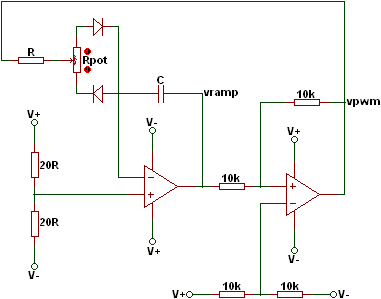
\includegraphics[scale=1]{02.PNG}\\
Los rectificadores controlados PWM son circuitos que convierten corriente alterna en corriente directa variable, los cuales incluyen una corrección de factor de potencia. La etapa de control presenta un acoplamiento con la línea de alimentación para generar un patrón PWM de los cuatro interruptores del puente rectificador. El acoplamiento con los elementos de potencia se realiza por medio de opto-acopladores de alta velocidad. Finalmente el puente rectificador se implementa por medio de 4 Mosfets para realizar el proceso de rectificación.\\

En convertidores de energía de corriente alterna esto se puede medir a través del factor de potencia del convertidor. Por definición este se mide por el cociente entre la potencia
promedio y la potencia aparente que demanda el circuito, el cual se puede también relacionar a la potencia reactiva del convertidor. Si la potencia reactiva es cero entonces el factor de potencia será unitario y la potencia entregada al convertidor será completamente utilizada.\\ 
En general, si la potencia reactiva es diferente de cero, entonces el factor de potencia será menor a la unidad. Así, idealmente se busca que todo convertidor de CA posea un factor de potencia cercano o inclusive la unidad. 
\section{Conclusiòn }
Los PWM son utilizados para rectificar la señal de onda y ademas poder varia su rango de trabago segun el voltage que emples, esto tiene grandes aplicaciones en los motores de corriente directa pues a demas de poder invertir el giro de estos pueden modificar su velocidad, ademas estos pueden ser usados para cruar amplificadores de sonido.
\cite{Biblio}
\bibliographystyle{apalike}
\bibliography{Biblio}
 

\end{document}